% A useful template for typesetting beautiful homework solutions. 
% Also check out Professor Matloff's guide: 
% http://heather.cs.ucdavis.edu/~matloff/LaTeX/HowToCreate.html.
\documentclass{article}

% Packages Used
\usepackage{fancyhdr} % Required for custom headers
\usepackage{lastpage} % Required to determine the last page for the footer
\usepackage{extramarks} % Required for headers and footers
\usepackage{graphicx} % Required to insert images
\usepackage{lipsum} % Used for inserting dummy 'Lorem ipsum' text into the template
\usepackage{comment}  % Used for multi-line commenting
\usepackage{booktabs} % For better looking tables
\usepackage{array}       % for better arrays (eg matrices) in maths
\usepackage{paralist}    % very flexible & customisable lists (eg. enumerate/itemize, etc.)
\usepackage{verbatim}  % adds environment for commenting out blocks of text & for better verbatim
\usepackage{subfig}      % make it possible to include more than one captioned figure/table in a single float
\usepackage{amsthm}   % make proofs look better
\usepackage{amsfonts}
\usepackage{amsmath}
\usepackage{amssymb}
\usepackage{eufrak}      % for fraktur fonts
\usepackage{mathabx}  % for \divides
\usepackage{enumerate} % to get lists enumerated with letters
\usepackage{hyperref}  % to get attractive URLs
\usepackage{bussproofs} % for setting proofs
\usepackage{etoolbox}
\usepackage{enumitem}
\usepackage{tikz}
\usepackage{cases}

% For theorem enviornment
\theoremstyle{definition}
\newtheorem{definition}{Definition}
\newtheorem{theorem}{Theorem}[section]
\newtheorem{corollary}{Corollary}[theorem]
\newtheorem{lemma}{Lemma}

\newtheorem{mathrule}{Rule}
\newtheorem{case}{Case}
\newtheorem{subcase}{Case}[case]

\theoremstyle{plain}
\newtheorem{example}{Example}
\newtheorem{problem}{Problem}[section]

% For improved end of proof formatting
\patchcmd{\endproof}  % <cmd>
  {\endtrivlist}               % <search>
  {\endtrivlist\par\nobreak\vspace*{\dimexpr-\baselineskip-\parskip}\nobreak\noindent\hrulefill}% <replace>
  {}{}                            % <succes><failure>

% Margins
\topmargin=-0.45in
\evensidemargin=0in
\oddsidemargin=0in
\textwidth=6.5in
\textheight=9.0in
\headsep=0.25in 

\linespread{1.1} % Line spacing

% Set up the header and footer
\pagestyle{fancy}
\lhead{PHY 9HC Spring 2016\\ UC Davis - Emilija Pantic} % Top left header
\chead{} % Top center header
\rhead{\firstxmark Anze Wang ID: 912777492\\PHY 9HC A02} % Top right header
\lfoot{\lastxmark} % Bottom left footer
\cfoot{} % Bottom center footer
\rfoot{Page\ \thepage\ of\ \pageref{LastPage}} % Bottom right footer

\setlength\parindent{10pt} % Removes all indentation from paragraphs

% Common boolean operators.
\newcommand*\AND{\wedge}
\newcommand*\OR{\vee}
\newcommand*\NOT{\neg}
\newcommand*\IMPLIES{\implies}
\newcommand*\XOR{\mathbin{\oplus}}


\begin{document}

\begin{center} \bf \LARGE Homework 2\\
\end{center}


\begin {enumerate}[itemindent=30pt,label=\bf Exercise {\arabic*}:]

\item Q3B.6\\
Suppose the light source for a two-slit interference experiment provides yellow light with a wavelength of \textbf{570 nm}. If this light is sent through a pair of slits separated by a distance \textbf{d=0.030 mm}, show that the angle between the bright spot corresponding to \textbf{n=0} and the bright spot corresponding to \textbf{n=1} is about \textbf{$1.1^{o}$}. If the display screen is a distance \textbf{D=2.4 m} from the slits, show that the distance between these bright spots on the screen is about \textbf{4.6 cm}.
\subitem (1)
\begin{align*}
	n \lambda &= d sin(\theta)\\
	\dfrac{n \lambda}{d} &= sin(\theta)\\
	\dfrac{n \lambda}{d} & = \frac{570 nm}{0.03 mm} = 0.019\\
 	sin(\theta) &= sin(1.1^{o}) = 0.019
\end{align*}
\subitem $\therefore$ the angle between the bright spot corresponding to n=0 and the bright spot corresponding to n=1 is about $1.1^{o}$.
\subitem (2)
 \begin{align*}
	y &= d sin(\theta) \\
	\quad\quad &= 2.4 * sin(1.1^{o}) \\
	\quad\quad &= 0.046 m\\
	\quad\quad &= 4.6 cm
\end{align*}
\subitem $\therefore$ If the display screen is a distance D=2.4 m from the slits, the distance between these bright spots on the screen is about 4.6 cm.
\item Q3B.8\\
As you are just about to round a corner, you hear two people talking some distance around the corner. One has a deep voice, and the other has a high voice. Which one more easily carries around the corner? Explain. \\
\subitem The deep voice has longer wave length because it has lower frequency. The long wave length can help it carry around the corner easier.
\newpage
\item Q3M.1 \\
You are setting up a pair of PA speakers on a field in preparation for an outdoor event. Each speaker is 0.65 m wide, and the speakers are separated by 8.2 m. To test the speakers, your coworker plays a single tone through the speakers whose frequency is 440 Hz. You are standing 52 m directly in front of the speakers and facing them. Roughly how far would you have to walk to your left or right to hear the sound amplitude drop almost to zero? How much farther would you have to go to hear the amplitude go back to its original strength? 
\begin{align*}
	\lambda &= \dfrac{v}{f} = \dfrac{340 m/s}{440 s^{-1}} = 0.77 m\\
	\theta_{0} &= sin^{-1}(\frac{\lambda}{d}) = sin^{-1}{\frac{0.77 m}{8.3 m}} = 0.09\quad rad\\
	\theta_{1} &= sin^{-1}(\frac{\lambda}{2d})= sin^{-1}{\frac{0.77 m}{2 * 8.3 m}} = 0.046\quad rad\\	   
	y_{0} &= D*tan(\theta_{0}) = 52* tan(0.046)  = 2.42 m \\ 
	y_{1} &= D*tan(\theta) = 52* tan(0.09) = 4.69 m
\end{align*}
\subitem I should walk 2.42 to hear the sound drop almost to zero, and I should walk 4.69m to hear the amplitude go back to original strength.
\\
\item Q3M.12\\ In J.R.R. Tolkien's The Lord of the Rings (volume 2, p. 32), Legolas the Elf claims to be able to accurately count horsemen and discern their hair color (yellow) 5 leagues away on a bright, sunny day. Make appropriate estimates and argue that Legolas must have very strange-looking eyes, have some means of nonvisual perception, or have made a lucky guess. (1 league $\approx$ 3.0 mi.)
\subitem According to wiki, I know that, in the sunny day, the diameter of human's pupil is 1.5mm.
\subitem Because the hair's color is yellow, the wave length of light is 520 nm
\subitem According to my suit-mate, the with of human's face is 20 cm
\subitem $\theta_{min} = sin^{-1}(\dfrac{1.22* \lambda}{a}) = sin^{-1}(\dfrac{1.22 520\;nm}{1.5 mm}) = 0.00042$
\subitem $\theta = 2*tan^{-1}(\dfrac{0.1}{24140}) = 8.285*10^{-6}$
\subitem $\because \theta < \theta_{min}$
\subitem $\therefore$ he cannot see it, if he does not have very strange-looking eyes.
\newpage
\item Q3D.1\\
Consider a two-slit interference experiment where you measure the amplitude of the combined wave at points a certain constant distance $D \gg d$ from the center of two slits separated by distance d. Using the superposition principle, show that the squared amplitude of the combined wave as a function of $\theta$ is 
$$[A(\theta)]^{2} = B cos^{2}(\pi \dfrac{d sin(\theta)}{\lambda} )\qquad(Q3.15)$$ \\
where λ is the waves' wavelength, and B is some positive constant. (Remember that the wave intensity is proportional to its squared amplitude.) You may assume that the sinusoidal circular waves created by each slit have approximately constant amplitude at all angles. (Hint: An appropriate trigonometric identity might help. Note that if $D \gg d$, the amplitude of the sinusoidal circular waves received from each slit will be roughly equal.) 
\begin{figure}[h]
\begin{center}
	\begin{tikzpicture}[scale=1.5]
    		\draw (0,0) -- (0,1.4);
        \draw (0,1.6) -- (0, 2.2);
		\draw (0, 2.4) -- (0, 3.8);
		\draw (5, 0) -- (5, 3.8);
        \draw (0, 2.3) -- (5, 3.3);
        \draw (0, 1.5) -- (5, 3.3);
        \draw[dashed] (0, 1.5) -- (5, 1.5);
        \draw[dashed] (0, 2.3) -- (0.27108 , 1.59759); 
		\draw (0.5,1.5) arc(0:20:0.5);
        \node at (2.5,2.2) {$r^{'}$};
        \node at (1,2.7) {r};
        \node at (-0.2, 1.9) {d};
        \node at (0.6, 1.6) {$\theta$};
        \node at (2.5, 1.3) {D};
        \node at (5.5, 2.4) {$Dtan(\theta)$};
	\end{tikzpicture}
\end{center}
\end{figure}
\subitem we have two wave function:
\begin{align*}
	&\Psi_{1}(r, t) = A sin(kr-\omega t)\\
	&\Psi_{2}(r, t) = A sin(k(r+d sin(\theta)) - \omega t)\\
	&\Psi_{1} + \Psi_{2} = A sin(kr-\omega t) + A sin(k(r+d sin(\theta)) - \omega t)\\
	&\qquad\quad\;\;\; = 2A\;cos(\dfrac{kdsin(\theta)}{2})\;sin(\dfrac{2r + dsin(\theta)}{2} k - \omega t)\\
	&|A(\theta)|^{2} = (2A\;cos(\dfrac{kdsin(\theta)}{2}))^{2}\\
	&\qquad \quad \;=B cos^{2}(\pi \dfrac{d sin(\theta)}{\lambda} )
\end{align*}

\newpage
\item Q3R.3\\
You are a detective interviewing someone who says that (while sitting on a porch that you know to be 600 ft away) he saw the masked suspect commit the crime in broad daylight. “How do you know it was the suspect?” you ask. “I clearly saw the 'MOM' that is tattooed on his upper arm.” “You're sure it was that particular tattoo and not some other tattoo?” “Yes, I'm sure,” the witness replies. The suspect's tattoo has letters that are 6 cm tall. Is the witness credible, or might he be framing the suspect? Justify your response and any estimates you might make. 
\begin{figure}[h]
	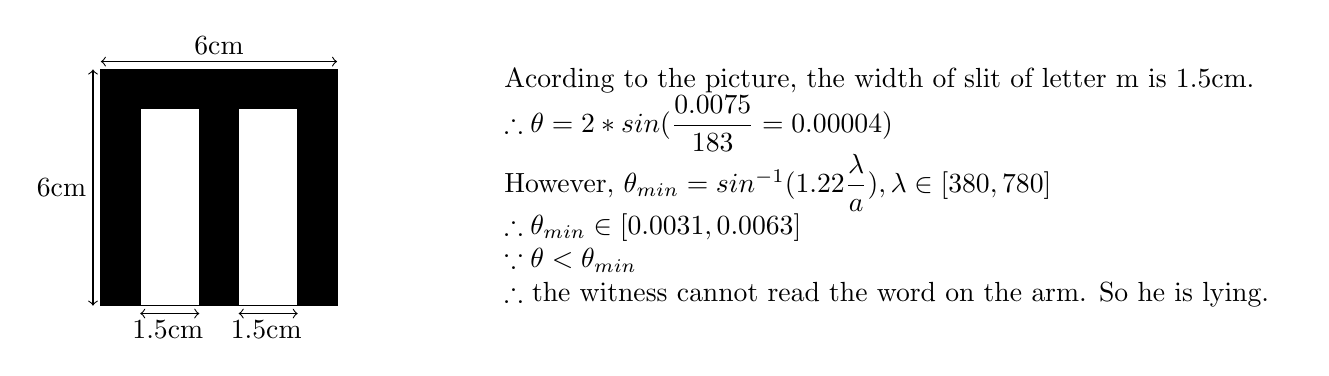
\begin{tikzpicture}
	
	\draw[black] (0,0) rectangle (3,3);
	\draw[fill = black] (0,0) rectangle (0.5,3);
	\draw[fill = black] (0,2.5) rectangle (3,3);
	\draw[fill = black] (1.25,0) rectangle (1.75,3);
	\draw[fill = black] (2.5,0) rectangle (3,3);
	\draw[<->] (0.5, -0.1) -- (1.25,-0.1);
	\draw[<->] (1.75, -0.1) -- (2.5,-0.1);
	\draw[<->] (-0.1, 0) -- (-0.1, 3);
	\draw[<->] (0, 3.1) -- (3,3.1);
	\node at (0.85, -0.3) {1.5cm};
	\node at (2.1, -0.3) {1.5cm};
	\node at (-0.5, 1.5) {6cm};
	\node at (1.5, 3.3){6cm}; 
	 \node [right, text width = 10cm, align = justify] at (5,1.5) {
            Acording to the picture, the width of slit of letter m is 1.5cm.\\
            $\therefore \theta = 2*sin(\dfrac{0.0075}{183} = 0.00004)$\\            
            However, $\theta_{min} = sin^{-1}(1.22 \dfrac{\lambda}{a}), \lambda \in [380, 780]$\\
            $\therefore \theta_{min} \in [0.0031, 0.0063]$ \\
            $\because \theta < \theta_{min}$ \\
            $\therefore$ the witness cannot read the word on the arm. So he is lying.
       
        };
	\end{tikzpicture}
\end{figure}

\end{enumerate}
\end{document}
